\part{Cuarto semestre}
\chapterimage{4.pdf}
\chapter{Geometría Analítica}


\section{Conceptos fundamentales} % (15 horas)
\subsection{Introducción y Plano Cartesiano}

\begin{definition}[Plano Cartesiano]
Es una herramienta esencial en la geometría analítica que permite representar gráficamente ecuaciones algebraicas. Está formado por dos ejes perpendiculares: el eje \( x \) (eje horizontal) y el eje \( y \) (eje vertical). Estos ejes dividen el plano en cuatro regiones conocidas como cuadrantes.
\end{definition} 

\begin{itemize}
    \item \textbf{Eje \( x \)}: También conocido como eje horizontal, mide la posición de un punto a lo largo de la dirección horizontal.
    \item \textbf{Eje \( y \)}: También conocido como eje vertical, mide la posición de un punto a lo largo de la dirección vertical.
    \item \textbf{Origen}: El punto de intersección de los ejes \( x \) y \( y \), denotado como \( (0,0) \).
\end{itemize}

\subsubsection{Sistema de Coordenadas}
Cada punto en el plano cartesiano se representa mediante un par ordenado \((x, y)\), donde \( x \) es la coordenada horizontal y \( y \) es la coordenada vertical.
\begin{center}
    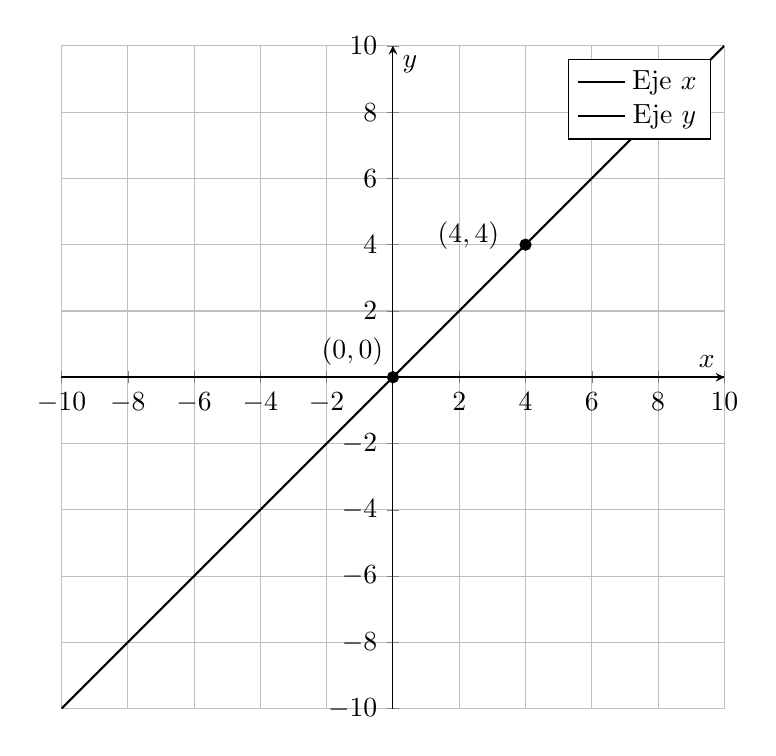
\begin{tikzpicture}
        \begin{axis}[
            axis lines = middle,
            xlabel = $x$,
            ylabel = {$y$},
            xmin = -10, xmax = 10,
            ymin = -10, ymax = 10,
            grid = major,
            width = 10cm,
            height = 10cm
        ]
        \addplot [
            domain=-10:10,
            samples=2,
            color=black,
            thick
        ]
        {0};
        \addlegendentry{Eje $x$}
        
        \addplot [
            domain=-10:10,
            samples=2,
            color=black,
            thick
        ]
        {x};
        \addlegendentry{Eje $y$}
        
        \draw [fill] (axis cs:0,0) circle [radius=2pt];
        \node at (axis cs:0,1.5) [anchor=north east] {$(0,0)$};
        \draw [fill] (axis cs:4,4) circle [radius=2pt];
        \node at (axis cs:3.5,5) [anchor=north east] {$(4,4)$};

        \end{axis}
    \end{tikzpicture}
\end{center}



\subsection{Distancia entre dos puntos}

La distancia entre dos puntos en el plano cartesiano se puede calcular utilizando la fórmula de la distancia. Si tenemos dos puntos \( A(x_1, y_1) \) y \( B(x_2, y_2) \), la distancia \( d \) entre ellos es:
\begin{equation}
    d = \sqrt{(x_2 - x_1)^2 + (y_2 - y_1)^2}
\end{equation}

\begin{example}
    Encuentra la distancia entre los puntos \( A(1, 2) \) y \( B(4, 6) \).
\[
d = \sqrt{(4 - 1)^2 + (6 - 2)^2} = \sqrt{3^2 + 4^2} = \sqrt{9 + 16} = \sqrt{25} = 5
\]
\end{example}

\begin{center}
    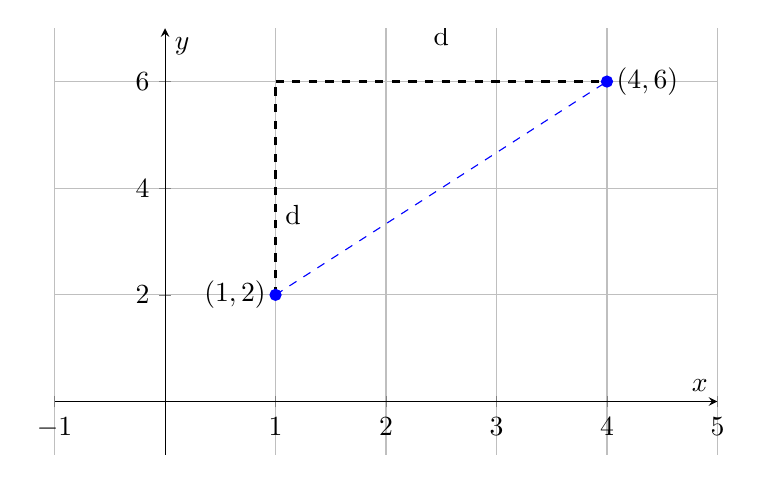
\begin{tikzpicture}
        \begin{axis}[
            axis lines = middle,
            xlabel = $x$,
            ylabel = $y$,
            xmin = -1, xmax = 5,
            ymin = -1, ymax = 7,
            grid = both,
            width=10cm, height=7cm
        ]
        \addplot [
            only marks,
            mark=*,
            color=blue
        ]
        coordinates {(1, 2) (4, 6)};
        
        \addplot [
            color=blue,
            dashed
        ]
        coordinates {(1, 2) (4, 6)};
        
        \node at (axis cs:1,2) [anchor=east] {$(1,2)$};
        \node at (axis cs:4,6) [anchor=west] {$(4,6)$};
        
        \draw[thick, dashed] (axis cs:1,2) -- (axis cs:1,6);
        \draw[thick, dashed] (axis cs:1,6) -- (axis cs:4,6);
        \node at (axis cs:1,3.5) [anchor=west] {d};
        \node at (axis cs:2.5,6.5) [anchor=south] {d};
        \end{axis}
    \end{tikzpicture}
\end{center}


\subsection{División de un segmento en una razón dada}

Para dividir un segmento de línea en una razón \( k:1 \), usamos la fórmula de la división de un segmento en coordenadas. Si el segmento une los puntos \( A(x_1, y_1) \) y \( B(x_2, y_2) \), el punto de división \( P(x, y) \) que divide el segmento en la razón \( k:1 \) es:
\begin{align}
    &x = \frac{kx_2 + x_1}{k + 1}\\
    &y = \frac{ky_2 + y_1}{k + 1}
\end{align}

\begin{example}
    Encuentra el punto que divide el segmento \( AB \) con \( A(1, 3) \) y \( B(4, 7) \) en la razón 2:1.
\[
x = \frac{2 \cdot 4 + 1}{2 + 1} = \frac{8 + 1}{3} = 3
\]
\[
y = \frac{2 \cdot 7 + 3}{2 + 1} = \frac{14 + 3}{3} = 5.67
\]
El punto es \( (3, 5.67) \).
\end{example}
\begin{center}
    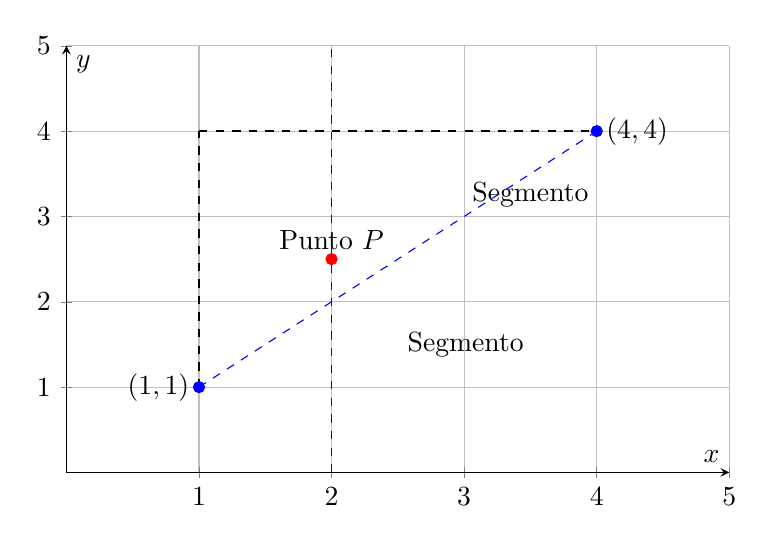
\begin{tikzpicture}
        \begin{axis}[
            axis lines = middle,
            xlabel = $x$,
            ylabel = $y$,
            xmin = 0, xmax = 5,
            ymin = 0, ymax = 5,
            grid = both,
            width=10cm, height=7cm
        ]
        \addplot [
            color=blue,
            mark=*,
            only marks
        ]
        coordinates {(1, 1) (4, 4)};
        
        \addplot [
            color=blue,
            dashed
        ]
        coordinates {(1, 1) (4, 4)};
        
        \addplot [
            color=red,
            mark=*,
            only marks
        ]
        coordinates {(2, 2.5)};
        
        \addplot [
            color=blue,
            dashed
        ]
        coordinates {(2, 0) (2, 5)};
        
        \node at (axis cs:1,1) [anchor=east] {$(1,1)$};
        \node at (axis cs:4,4) [anchor=west] {$(4,4)$};
        \node at (axis cs:2,2.5) [anchor=south] {Punto $P$};
        
        \draw[thick, dashed] (axis cs:1,1) -- (axis cs:1,4);
        \draw[thick, dashed] (axis cs:1,4) -- (axis cs:4,4);
        \node at (axis cs:2.5,1.5) [anchor=west] {Segmento};
        \node at (axis cs:3.5,3) [anchor=south] {Segmento};
        \end{axis}
    \end{tikzpicture}
\end{center}

\subsection{Punto medio de un segmento}

El punto medio de un segmento que une los puntos \( A(x_1, y_1) \) y \( B(x_2, y_2) \) se calcula como:
\begin{equation}
    M = \left( \frac{x_1 + x_2}{2}, \frac{y_1 + y_2}{2} \right)
\end{equation}

\begin{example}
    Encuentra el punto medio del segmento que une \( A(1, 2) \) y \( B(4, 6) \).
\[
M = \left( \frac{1 + 4}{2}, \frac{2 + 6}{2} \right) = \left( \frac{5}{2}, \frac{8}{2} \right) = \left( 2.5, 4 \right)
\]

\end{example}

\begin{center}
    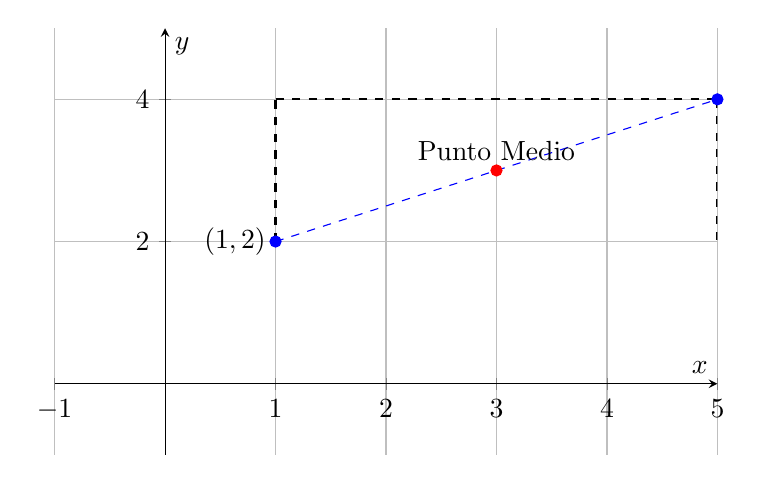
\begin{tikzpicture}
        \begin{axis}[
            axis lines = middle,
            xlabel = $x$,
            ylabel = $y$,
            xmin = -1, xmax = 5,
            ymin = -1, ymax = 5,
            grid = both,
            width=10cm, height=7cm
        ]
        \addplot [
            color=blue,
            mark=*,
            only marks
        ]
        coordinates {(1, 2) (5, 4)};
        
        \addplot [
            color=blue,
            dashed
        ]
        coordinates {(1, 2) (5, 4)};
        
        \addplot [
            color=red,
            mark=*,
            only marks
        ]
        coordinates {(3, 3)};
        
        \node at (axis cs:1,2) [anchor=east] {$(1,2)$};
        \node at (axis cs:5,4) [anchor=west] {$(5,4)$};
        \node at (axis cs:3,3) [anchor=south] {Punto Medio};
        
        \draw[thick, dashed] (axis cs:1,2) -- (axis cs:1,4);
        \draw[thick, dashed] (axis cs:1,4) -- (axis cs:5,4);
        \draw[thick, dashed] (axis cs:5,4) -- (axis cs:5,2);
        \end{axis}
    \end{tikzpicture}
\end{center} 
\subsection{Conceptos de ángulo de inclinación y pendiente}

El ángulo de inclinación \(\theta\) de una recta con pendiente \( m \) se puede encontrar mediante:
\begin{equation}
    \tan(\theta) = m \implies \theta = \arctan(m)
\end{equation}
La pendiente \( m \) de una recta en la forma \( y = mx + b \) es el coeficiente \( m \).

\begin{example}
    Para una recta con ecuación \( y = 2x + 1 \), la pendiente es \( 2 \). El ángulo de inclinación es:
\[
\theta = \arctan(2) \approx 63.43^\circ
\]
\begin{center}
    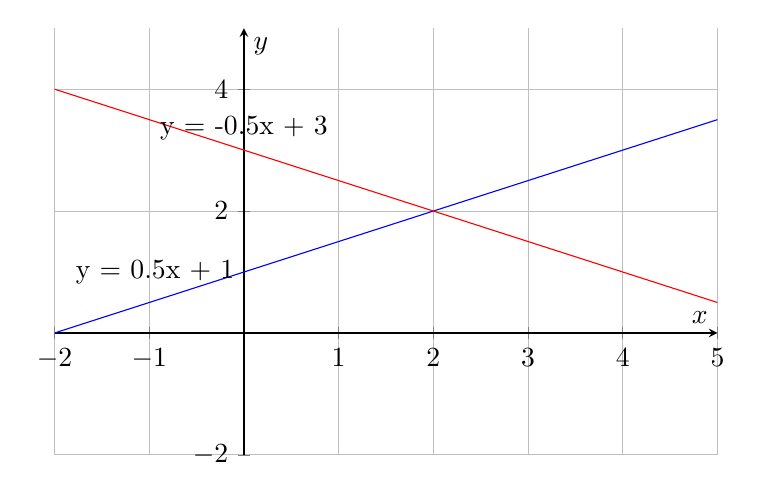
\begin{tikzpicture}
        \begin{axis}[
            axis lines = middle,
            xlabel = $x$,
            ylabel = $y$,
            xmin = -2, xmax = 5,
            ymin = -2, ymax = 5,
            grid = both,
            width=10cm, height=7cm
        ]
        \addplot [
            color=blue,
            domain=-2:5,
            samples=100
        ]
        {0.5*x + 1};
        
        \addplot [
            color=red,
            domain=-2:5,
            samples=100
        ]
        {-0.5*x + 3};
        
        \node at (axis cs:0,1) [anchor=east] {y = 0.5x + 1};
        \node at (axis cs:0,3) [anchor=south] {y = -0.5x + 3};
    \end{axis}
    \end{tikzpicture}
\end{center}
\end{example}
\subsection{Ángulo entre dos rectas}

El ángulo \(\phi\) entre dos rectas con pendientes \( m_1 \) y \( m_2 \) se calcula usando:
\begin{equation}
    \tan(\phi) = \left| \frac{m_1 - m_2}{1 + m_1m_2} \right|
\end{equation}

\begin{example}
    Encuentra el ángulo entre las rectas \( y = 2x + 1 \) y \( y = -\frac{1}{2}x + 3 \).
\[
\tan(\phi) = \left| \frac{2 - (-\frac{1}{2})}{1 + 2 \cdot (-\frac{1}{2})} \right| = \left| \frac{2 + \frac{1}{2}}{1 - 1} \right| = \text{indeterminado}
\]
Las rectas son perpendiculares.
\begin{center}
    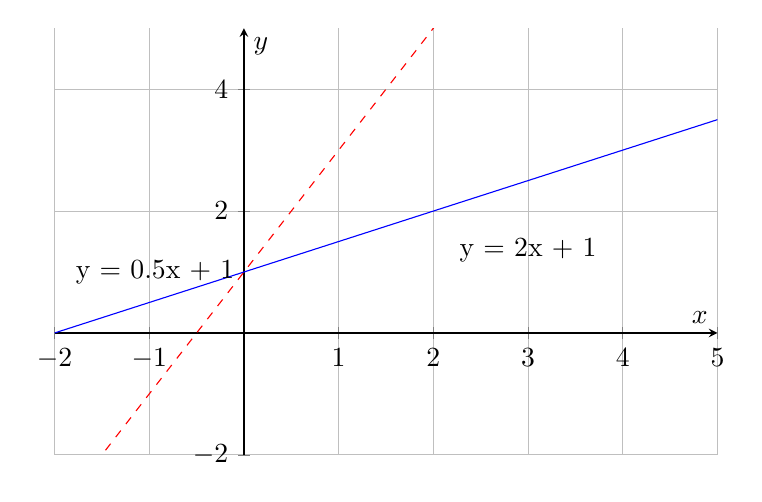
\begin{tikzpicture}
        \begin{axis}[
            axis lines = middle,
            xlabel = $x$,
            ylabel = $y$,
            xmin = -2, xmax = 5,
            ymin = -2, ymax = 5,
            grid = both,
            width=10cm, height=7cm
        ]
        \addplot [
            color=blue,
            domain=-2:5,
            samples=100
        ]
        {0.5*x + 1};
        
        \addplot [
            color=red,
            domain=-2:5,
            samples=100,
            dashed
        ]
        {2*x + 1};
        
        \node at (axis cs:0,1) [anchor=east] {y = 0.5x + 1};
        \node at (axis cs:3,1) [anchor=south] {y = 2x + 1};
    \end{axis}
    \end{tikzpicture}
\end{center}
\end{example}

\subsection{Paralelismo y Perpendicularidad}

Dos rectas son paralelas si tienen la misma pendiente \( m \). Son perpendiculares si el producto de sus pendientes es \(-1\):
\begin{equation}
    m_1 \cdot m_2 = - 1
\end{equation}

\begin{example}
    Las rectas \( y = 3x + 2 \) y \( y = -\frac{1}{3}x + 4 \) son perpendiculares porque:
\[
3 \cdot \left(-\frac{1}{3}\right) = -1
\]
\end{example}

\begin{center}
    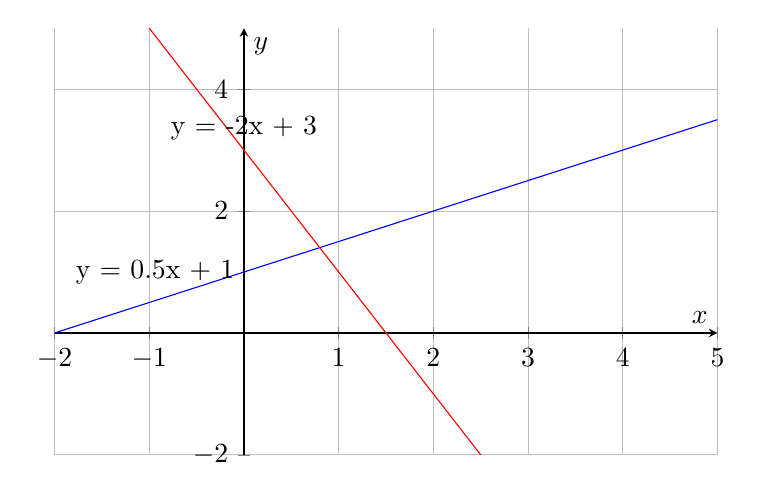
\begin{tikzpicture}
        \begin{axis}[
            axis lines = middle,
            xlabel = $x$,
            ylabel = $y$,
            xmin = -2, xmax = 5,
            ymin = -2, ymax = 5,
            grid = both,
            width=10cm, height=7cm
        ]
        \addplot [
            color=blue,
            domain=-2:5,
            samples=100
        ]
        {0.5*x + 1};
        
        \addplot [
            color=red,
            domain=-2:5,
            samples=100
        ]
        {-2*x + 3};
        
        \node at (axis cs:0,1) [anchor=east] {y = 0.5x + 1};
        \node at (axis cs:0,3) [anchor=south] {y = -2x + 3};
    \end{axis}
    \end{tikzpicture}
\end{center}
\subsection{Cálculo de Áreas de polígonos}


\subsubsection{Triángulo}
Para calcular el área de un triángulo con vértices en $(x_1, y_1)$, $(x_2, y_2)$, y $(x_3, y_3)$, usamos la fórmula:

\[ \text{Área} = \frac{1}{2} \left| x_1(y_2 - y_3) + x_2(y_3 - y_1) + x_3(y_1 - y_2) \right| \]

\begin{center}
    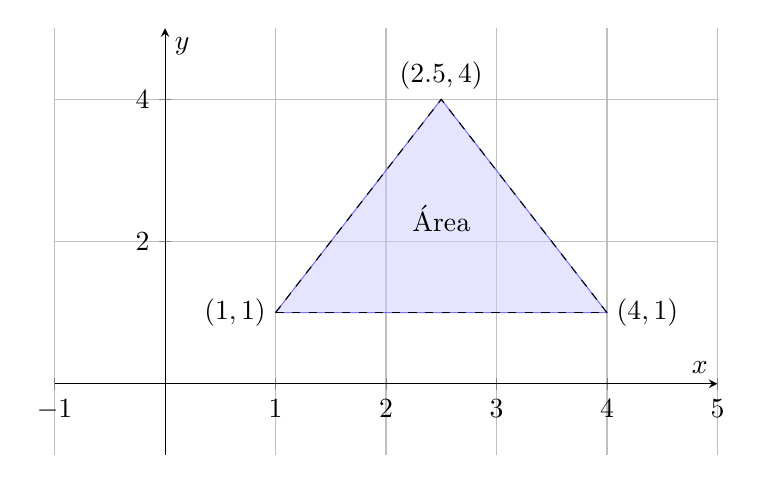
\begin{tikzpicture}
        \begin{axis}[
            axis lines = middle,
            xlabel = $x$,
            ylabel = $y$,
            xmin = -1, xmax = 5,
            ymin = -1, ymax = 5,
            grid = both,
            width=10cm, height=7cm
        ]
        \addplot [
            color=blue,
            fill=blue!20,
            opacity=0.5
        ]
        coordinates {(1,1) (4,1) (2.5,4) (1,1)};
        
        \node at (axis cs:1,1) [anchor=east] {$(1,1)$};
        \node at (axis cs:4,1) [anchor=west] {$(4,1)$};
        \node at (axis cs:2.5,4) [anchor=south] {$(2.5,4)$};
        \node at (axis cs:2.5,2) [anchor=south] {Área};
        
        \draw[dashed] (axis cs:1,1) -- (axis cs:4,1);
        \draw[dashed] (axis cs:1,1) -- (axis cs:2.5,4);
        \draw[dashed] (axis cs:4,1) -- (axis cs:2.5,4);
    \end{axis}
    \end{tikzpicture}
\end{center}

\subsubsection{Cálculo del Área de un Triángulo con Determinantes}

Para calcular el área de un triángulo con vértices en $(x_1, y_1)$, $(x_2, y_2)$, y $(x_3, y_3)$, usamos la fórmula:

\[ \text{Área} = \frac{1}{2} \left| \text{det} \begin{pmatrix}
x_1 & y_1 & 1 \\
x_2 & y_2 & 1 \\
x_3 & y_3 & 1
\end{pmatrix} \right| \]

donde \(\text{det}\) denota el determinante de la matriz.

\begin{example}
    Consideremos un triángulo con vértices en $(1,1)$, $(4,1)$, y $(2.5,4)$. Aplicamos la fórmula:

1. Escribimos la matriz:

\[
\begin{pmatrix}
1 & 1 & 1 \\
4 & 1 & 1 \\
2.5 & 4 & 1
\end{pmatrix}
\]

2. Calculamos el determinante:

\[
\text{det} \begin{pmatrix}
1 & 1 & 1 \\
4 & 1 & 1 \\
2.5 & 4 & 1
\end{pmatrix} = 1 \cdot \left(1 \cdot 1 - 1 \cdot 4 \right) - 1 \cdot \left(4 \cdot 1 - 1 \cdot 2.5 \right) + 1 \cdot \left(4 \cdot 4 - 1 \cdot 2.5 \right)
\]

\[
= 1 \cdot (1 - 4) - 1 \cdot (4 - 2.5) + 1 \cdot (16 - 2.5)
\]

\[
= 1 \cdot (-3) - 1 \cdot 1.5 + 1 \cdot 13.5
\]

\[
= -3 - 1.5 + 13.5
\]

\[
= 9
\]

3. Calculamos el área:

\[
\text{Área} = \frac{1}{2} \left| 9 \right| = \frac{9}{2} = 4.5
\]

\begin{center}
    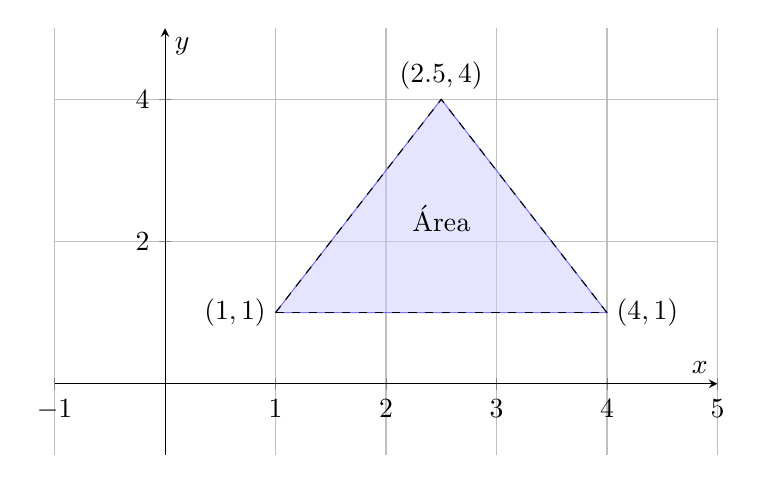
\begin{tikzpicture}
        \begin{axis}[
            axis lines = middle,
            xlabel = $x$,
            ylabel = $y$,
            xmin = -1, xmax = 5,
            ymin = -1, ymax = 5,
            grid = both,
            width=10cm, height=7cm
        ]
        \addplot [
            color=blue,
            fill=blue!20,
            opacity=0.5
        ]
        coordinates {(1,1) (4,1) (2.5,4) (1,1)};
        
        \node at (axis cs:1,1) [anchor=east] {$(1,1)$};
        \node at (axis cs:4,1) [anchor=west] {$(4,1)$};
        \node at (axis cs:2.5,4) [anchor=south] {$(2.5,4)$};
        \node at (axis cs:2.5,2) [anchor=south] {Área};
        
        \draw[dashed] (axis cs:1,1) -- (axis cs:4,1);
        \draw[dashed] (axis cs:1,1) -- (axis cs:2.5,4);
        \draw[dashed] (axis cs:4,1) -- (axis cs:2.5,4);
    \end{axis}
    \end{tikzpicture}
\end{center}

\end{example}


\subsubsection{Cuadrado}
Para un cuadrado con vértices en $(x_1, y_1)$, $(x_2, y_2)$, $(x_3, y_3)$, y $(x_4, y_4)$, el área se calcula usando la longitud del lado:

\[ \text{lado} = \sqrt{(x_2 - x_1)^2 + (y_2 - y_1)^2} \]
\[ \text{Área} = \text{lado}^2 \]

\begin{center}
    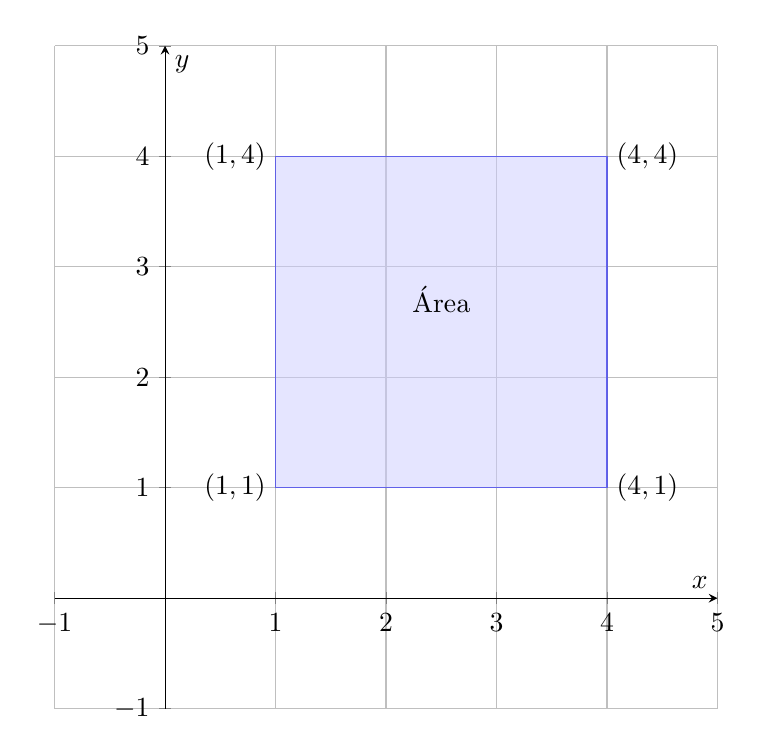
\begin{tikzpicture}
        \begin{axis}[
            axis lines = middle,
            xlabel = $x$,
            ylabel = $y$,
            xmin = -1, xmax = 5,
            ymin = -1, ymax = 5,
            grid = both,
            width=10cm, height=10cm
        ]
        \addplot [
            color=blue,
            fill=blue!20,
            opacity=0.5
        ]
        coordinates {(1,1) (4,1) (4,4) (1,4) (1,1)};
        
        \node at (axis cs:1,1) [anchor=east] {$(1,1)$};
        \node at (axis cs:4,1) [anchor=west] {$(4,1)$};
        \node at (axis cs:4,4) [anchor=west] {$(4,4)$};
        \node at (axis cs:1,4) [anchor=east] {$(1,4)$};
        \node at (axis cs:2.5,2.5) [anchor=south] {Área};
    \end{axis}
    \end{tikzpicture}
\end{center}

\subsubsection{Rectángulo}
Para un rectángulo con vértices en $(x_1, y_1)$, $(x_2, y_2)$, $(x_3, y_3)$, y $(x_4, y_4)$:

\[ \text{base} = \sqrt{(x_2 - x_1)^2 + (y_2 - y_1)^2} \]
\[ \text{altura} = \sqrt{(x_3 - x_2)^2 + (y_3 - y_2)^2} \]
\[ \text{Área} = \text{base} \times \text{altura} \]

\begin{center}
    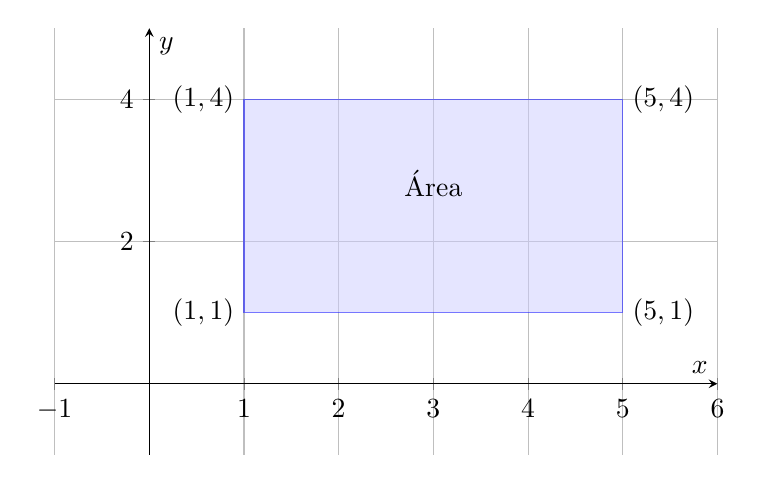
\begin{tikzpicture}
        \begin{axis}[
            axis lines = middle,
            xlabel = $x$,
            ylabel = $y$,
            xmin = -1, xmax = 6,
            ymin = -1, ymax = 5,
            grid = both,
            width=10cm, height=7cm
        ]
        \addplot [
            color=blue,
            fill=blue!20,
            opacity=0.5
        ]
        coordinates {(1,1) (5,1) (5,4) (1,4) (1,1)};
        
        \node at (axis cs:1,1) [anchor=east] {$(1,1)$};
        \node at (axis cs:5,1) [anchor=west] {$(5,1)$};
        \node at (axis cs:5,4) [anchor=west] {$(5,4)$};
        \node at (axis cs:1,4) [anchor=east] {$(1,4)$};
        \node at (axis cs:3,2.5) [anchor=south] {Área};
    \end{axis}
    \end{tikzpicture}
\end{center}

\subsubsection{Trapecio}
Para un trapecio con bases paralelas, se calcula el área usando las bases y la altura:

\[ \text{Área} = \frac{1}{2} \left( b_1 + b_2 \right) \times h \]

\begin{center}
    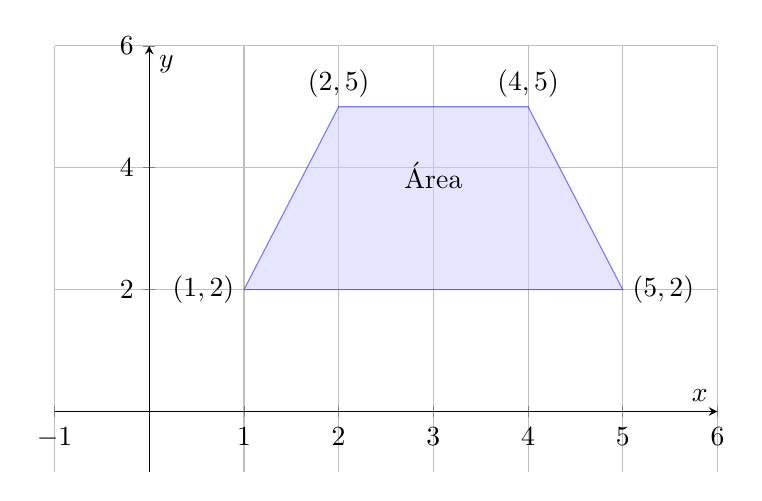
\begin{tikzpicture}
        \begin{axis}[
            axis lines = middle,
            xlabel = $x$,
            ylabel = $y$,
            xmin = -1, xmax = 6,
            ymin = -1, ymax = 6,
            grid = both,
            width=10cm, height=7cm
        ]
        \addplot [
            color=blue,
            fill=blue!20,
            opacity=0.5
        ]
        coordinates {(1,2) (5,2) (4,5) (2,5) (1,2)};
        
        \node at (axis cs:1,2) [anchor=east] {$(1,2)$};
        \node at (axis cs:5,2) [anchor=west] {$(5,2)$};
        \node at (axis cs:4,5) [anchor=south] {$(4,5)$};
        \node at (axis cs:2,5) [anchor=south] {$(2,5)$};
        \node at (axis cs:3,3.5) [anchor=south] {Área};
    \end{axis}
    \end{tikzpicture}
\end{center}

\subsubsection{Polígono Regular}
Para un polígono regular con \(n\) lados de longitud \(l\):

\[ \text{Área} = \frac{n \times l^2}{4 \tan\left(\frac{\pi}{n}\right)} \]

\begin{center}
    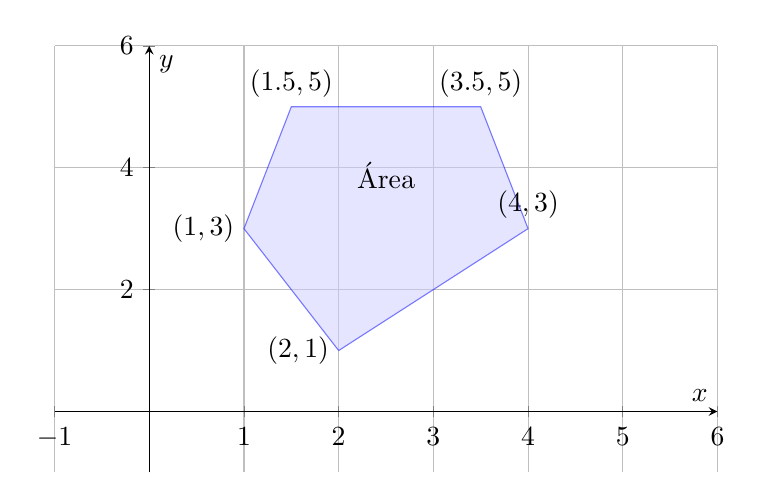
\begin{tikzpicture}
        \begin{axis}[
            axis lines = middle,
            xlabel = $x$,
            ylabel = $y$,
            xmin = -1, xmax = 6,
            ymin = -1, ymax = 6,
            grid = both,
            width=10cm, height=7cm
        ]
        \addplot [
            color=blue,
            fill=blue!20,
            opacity=0.5
        ]
        coordinates {(2,1) (4,3) (3.5,5) (1.5,5) (1,3) (2,1)};
        
        \node at (axis cs:2,1) [anchor=east] {$(2,1)$};
        \node at (axis cs:4,3) [anchor=south] {$(4,3)$};
        \node at (axis cs:3.5,5) [anchor=south] {$(3.5,5)$};
        \node at (axis cs:1.5,5) [anchor=south] {$(1.5,5)$};
        \node at (axis cs:1,3) [anchor=east] {$(1,3)$};
        \node at (axis cs:2.5,3.5) [anchor=south] {Área};
    \end{axis}
    \end{tikzpicture}
\end{center}







\section{Línea recta} %(15 horas)
\subsection{Definición de línea recta como lugar geométrico}

\begin{definition}[Linea Recta]
    Una línea recta se define como el lugar geométrico de los puntos que satisfacen una ecuación lineal.
\end{definition}
En términos sencillos, una línea recta es una colección infinita de puntos que se extienden en dos direcciones sin fin y sin curvatura.
\subsection{Ecuación de la Recta Conociendo las Coordenadas de un Punto Localizado en Ella y la Pendiente de la Misma}

Si conocemos un punto \((x_1, y_1)\) y la pendiente \(m\) de la recta, la ecuación de la recta se puede expresar en la forma punto-pendiente:
\begin{equation}
    Y - y_1 = m (X - x_1)
\end{equation}

\begin{example}
    Dada la pendiente \(m = 2\) y el punto \((1, 3)\), la ecuación de la recta es:

    \[
    y - 3 = 2 (x - 1) \quad \text{o} \quad y = 2x + 1
    \]
    \begin{center}
        \begin{tikzpicture}
            \begin{axis}[
                axis lines = middle,
                xlabel = $x$,
                ylabel = $y$,
                xmin = -5, xmax = 5,
                ymin = -5, ymax = 5,
                samples = 100,
                domain = -5:5
            ]
            \addplot [
                color=blue,
                thick
            ]
            {2*x + 1};
            \addlegendentry{$y = 2x + 1$}
            \end{axis}
        \end{tikzpicture}
    \end{center}

    \begin{center}
        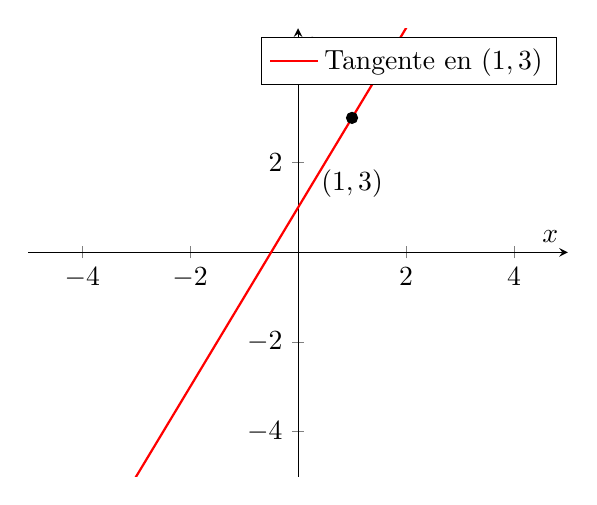
\begin{tikzpicture}
            \begin{axis}[
                axis lines = middle,
                xlabel = $x$,
                ylabel = $y$,
                xmin = -5, xmax = 5,
                ymin = -5, ymax = 5,
                samples = 100
            ]
            \addplot [
                color=red,
                thick
            ]
            {2*(x - 1) + 3}; % y - y1 = m(x - x1)
            \addlegendentry{Tangente en $(1,3)$}
            \draw [fill] (axis cs:1,3) circle [radius=2pt];
            \node at (axis cs:1,1) [anchor=south] {$(1, 3)$};
            \end{axis}
        \end{tikzpicture}
    \end{center}
\end{example}
\subsection{Ecuación de la Recta Dados Dos Puntos Distintos}

Si tenemos dos puntos \((x_1, y_1)\) y \((x_2, y_2)\), la pendiente \(m\) de la recta que pasa por estos puntos se calcula como:
\begin{equation}
    m = \frac{y_2 - y_1}{x_2 - x_1}
\end{equation}

Luego, usamos la ecuación punto-pendiente con uno de los puntos para obtener la ecuación de la recta.

\begin{example}
Para los puntos \((2, 1)\) y \((4, 3)\):

\[
m = \frac{3 - 1}{4 - 2} = 1
\]

La ecuación es:

\[
y - 1 = 1(x - 2) \quad \text{o} \quad y = x - 1
\]

\begin{center}
    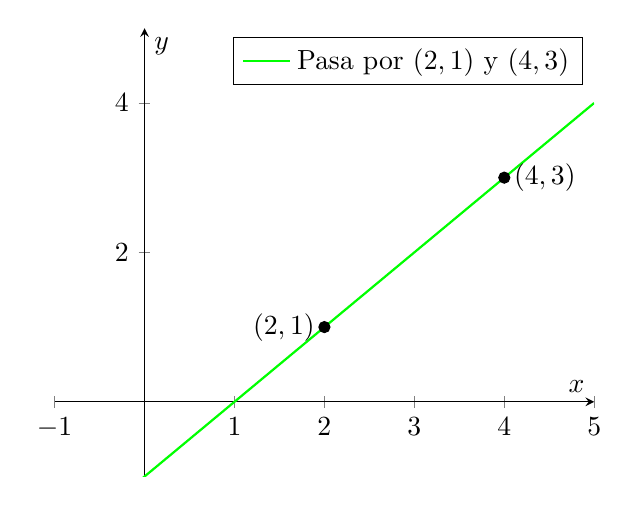
\begin{tikzpicture}
        \begin{axis}[
            axis lines = middle,
            xlabel = $x$,
            ylabel = $y$,
            xmin = -1, xmax = 5,
            ymin = -1, ymax = 5,
            samples = 100
        ]
        \addplot [
            color=green,
            thick
        ]
        {1*(x - 2) + 1}; % y - y1 = m(x - x1) with points (2,1) and (4,3)
        \addlegendentry{Pasa por $(2,1)$ y $(4,3)$}
        \draw [fill] (axis cs:2,1) circle [radius=2pt];
        \draw [fill] (axis cs:4,3) circle [radius=2pt];
        \node at (axis cs:2,1) [anchor=east] {$(2, 1)$};
        \node at (axis cs:4,3) [anchor=west] {$(4, 3)$};
        \end{axis}
    \end{tikzpicture}
\end{center}
\end{example}

\subsection{Ecuación de la Recta Dadas su Pendiente y su Ordenada al Origen}

La ecuación de la recta en forma pendiente-ordenada al origen es:
\begin{equation}
    y = mx + b
\end{equation}

donde \(m\) es la pendiente y \(b\) es la ordenada al origen.

\begin{example}
    Si la pendiente es \(3\) y la ordenada al origen es \(-2\), la ecuación de la recta es:

\[
y = 3x - 2
\]

\begin{center}
    \begin{tikzpicture}
        \begin{axis}[
            axis lines = middle,
            xlabel = $x$,
            ylabel = $y$,
            xmin = -5, xmax = 5,
            ymin = -5, ymax = 5,
            samples = 100
        ]
        \addplot [
            color=purple,
            thick
        ]
        {3*x - 2}; % y = mx + b
        \addlegendentry{$y = 3x - 2$}
        \end{axis}
    \end{tikzpicture}
\end{center}
\end{example}

\subsection{Ecuación Simétrica de la Recta}

La ecuación simétrica de una recta en el espacio, dado un punto \((x_0, y_0)\) y direcciones \((a, b)\), es:
\begin{equation}
    \frac{x - x_0}{a} = \frac{y - y_0}{b}
\end{equation}

\begin{example}
Para la recta con punto \((2, 1)\) y dirección \((3, 4)\), la ecuación es:
\[
\frac{x - 2}{3} = \frac{y - 1}{4}
\]
\begin{center}
    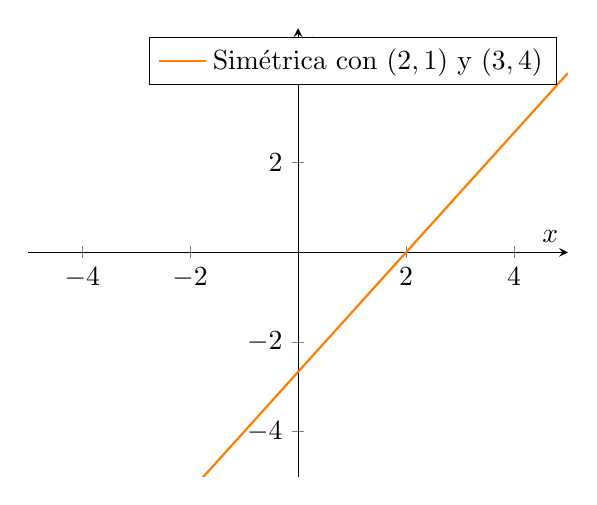
\begin{tikzpicture}
        \begin{axis}[
            axis lines = middle,
            xlabel = $x$,
            ylabel = $y$,
            xmin = -5, xmax = 5,
            ymin = -5, ymax = 5,
            samples = 100
        ]
        \addplot [
            color=orange,
            thick
        ]
        {4*(x - 2) / 3}; % (x - x0) / a = (y - y0) / b
        \addlegendentry{Simétrica con $(2,1)$ y $(3,4)$}
        \end{axis}
    \end{tikzpicture}
\end{center}
\end{example}


\subsection{Ecuación General de la Recta}

La ecuación general de una recta se puede expresar como:
\begin{equation}
    Ax + By + C = 0
\end{equation}

donde \(A\), \(B\), y \(C\) son constantes.


\subsection{Distancia de un Punto a una Recta}

La distancia \(d\) entre un punto \((x_0, y_0)\) y una recta \(Ax + By + C = 0\) se calcula con la fórmula:

\[
d = \frac{|Ax_0 + By_0 + C|}{\sqrt{A^2 + B^2}}
\]

\begin{example}
    La distancia entre el punto \((1, -2)\) y la recta \(3x - 2y + 6 = 0\) se calcula de la siguiente manera:

\[
d = \frac{|3 \cdot 1 - 2 \cdot (-2) + 6|}{\sqrt{3^2 + (-2)^2}} = \frac{|3 + 4 + 6|}{\sqrt{9 + 4}} = \frac{13}{\sqrt{13}} = \sqrt{13}
\]

\begin{center}
    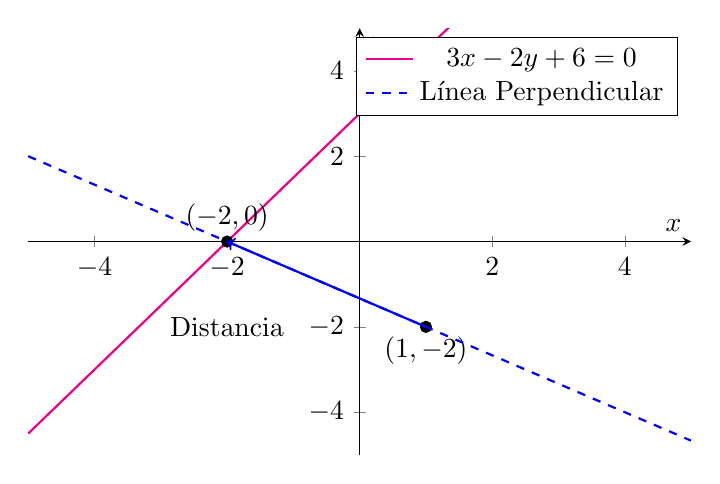
\begin{tikzpicture}
        \begin{axis}[
            axis lines = middle,
            xlabel = $x$,
            ylabel = $y$,
            xmin = -5, xmax = 5,
            ymin = -5, ymax = 5,
            samples = 100,
            width = 10cm,
            height = 7cm
        ]
        % Ecuación de la recta
        \addplot [
            color=magenta,
            thick
        ]
        {3/2*x + 3}; % Reescribiendo 3x - 2y + 6 = 0 en la forma y = mx + b
        \addlegendentry{$3x - 2y + 6 = 0$}
        
        % Puntos
        \draw [fill] (axis cs:1,-2) circle [radius=2pt];
        \node at (axis cs:1,-2) [anchor=north] {$(1, -2)$};
        
        % Coordenadas en el eje Y
        \draw [fill] (axis cs:-2,0) circle [radius=2pt];
        \node at (axis cs:-2,0) [anchor=south] {$(-2, 0)$};
        
        % Línea perpendicular
        \addplot [
            color=blue,
            thick,
            dashed
        ]
        {(-2/3)*(x - 1) - 2}; % La línea perpendicular al punto
        \addlegendentry{Línea Perpendicular}
        
        % Distancia desde el punto hasta la recta
        \draw [blue, thick, ->] (axis cs:1,-2) -- (axis cs:-2,0);
        \node at (axis cs:-1, -2) [anchor=east] {Distancia};
        \end{axis}
    \end{tikzpicture}
\end{center}
\end{example}





\section{Circunferencia} %(10.5 horas)
\subsection{Definición de la circunferencia como lugar geométrico}
La circunferencia es el conjunto de todos los puntos en un plano que están a una distancia fija, llamada radio, de un punto fijo, llamado centro. 

\subsection{Ecuación Ordinaria de la Circunferencia y su Gráfica}

La ecuación ordinaria de una circunferencia con centro en \((h, k)\) y radio \(r\) es:
\begin{equation}
    (x - h)^2 + (y - k)^2 = r^2
\end{equation}

% \begin{center}
%     \begin{tikzpicture}
%         \begin{axis}[
%             axis lines = middle,
%             xlabel = $x$,
%             ylabel = $y$,
%             xmin = -5, xmax = 5,
%             ymin = -5, ymax = 5,
%             width = 10cm,
%             height = 10cm
%         ]
%         \draw (1,-2) circle (2) ;
%         \addplot [
%             domain=0:360,
%             samples=100,
%             color=blue,
%             thick
%         ]{2 * sin(x) + 2 * cos(x)}; % Ecuación parametrizada
%         \addlegendentry{Circunferencia $(x-1)^2 + (y+2)^2 = 4$}
        
%         \draw [fill] (axis cs:1,-2) circle [radius=2pt];
%         \node at (axis cs:1,-2) [anchor=east] {Centro $(1, -2)$};
        
%         \node at (axis cs:2,-2) [anchor=south] {Radio = 2};
%         \draw [dashed] (axis cs:1,-2) -- (axis cs:3,-2);
%     \end{axis}
%     \end{tikzpicture}
% \end{center}

\subsection{Ecuación General de la Circunferencia}

La ecuación general de la circunferencia se obtiene expandiendo y simplificando la ecuación ordinaria:

\[
(x - h)^2 + (y - k)^2 = r^2
\]

Expandiendo:

\[
x^2 - 2hx + h^2 + y^2 - 2ky + k^2 = r^2
\]

Reorganizando:

\[
x^2 + y^2 - 2hx - 2ky + (h^2 + k^2 - r^2) = 0
\]

\subsection{Propiedades de la Circunferencia}

\begin{itemize}
    \item La circunferencia es un conjunto de puntos equidistantes de un punto central.
    \item Todos los radios de una circunferencia tienen la misma longitud.
    \item La longitud de la circunferencia es \(2 \pi r\).
    \item El área dentro de la circunferencia es \(\pi r^2\).
\end{itemize}

\subsection{Ecuación de la Circunferencia Determinada a partir de Condiciones Dadas}

Para determinar la ecuación de una circunferencia con condiciones dadas, por ejemplo, si conocemos el centro \((h, k)\) y un punto sobre la circunferencia \((x_1, y_1)\), primero calculamos el radio:
\begin{equation}
    r = \sqrt{(x_1 - h)^2 + (y_1 - k)^2}
\end{equation}

Luego, usamos la ecuación ordinaria:

\[
(x - h)^2 + (y - k)^2 = r^2
\]

ejemplo

Supongamos que el centro de la circunferencia es \((2, 3)\) y pasa por el punto \((4, 7)\). Calculamos el radio:

\[
r = \sqrt{(4 - 2)^2 + (7 - 3)^2} = \sqrt{4 + 16} = \sqrt{20} = 2\sqrt{5}
\]

La ecuación de la circunferencia es:

\[
(x - 2)^2 + (y - 3)^2 = (2\sqrt{5})^2
\]

\[
(x - 2)^2 + (y - 3)^2 = 20
\]

% \begin{center}
%     \begin{tikzpicture}
%         \begin{axis}[
%             axis lines = middle,
%             xlabel = $x$,
%             ylabel = $y$,
%             xmin = 0, xmax = 6,
%             ymin = 0, ymax = 8,
%             width = 10cm,
%             height = 10cm
%         ]
%         \addplot [
%             domain=0:360,
%             samples=100,
%             color=red,
%             thick
%         ]
%         {5 * sin(x) + 3 * cos(x)}; % Ecuación parametrizada
%         \addlegendentry{Circunferencia $(x-2)^2 + (y-3)^2 = 20$}
        
%         \draw [fill] (axis cs:2,3) circle [radius=2pt];
%         \node at (axis cs:2,3) [anchor=east] {Centro $(2, 3)$};
        
%         \draw [fill] (axis cs:4,7) circle [radius=2pt];
%         \node at (axis cs:4,7) [anchor=south] {Punto $(4, 7)$};
        
%         \node at (axis cs:2,6) [anchor=east] {Radio $2\sqrt{5}$};
%         \draw [dashed] (axis cs:2,3) -- (axis cs:4,7);
%     \end{axis}
%     \end{tikzpicture}
% \end{center}






\section{Parábola} %(9 horas)
\subsection{Definición de la parábola como lugar geométrico.}
Una \textbf{parábola} es el conjunto de todos los puntos en el plano que están a la misma distancia de un punto fijo llamado \textit{foco} y una línea fija llamada \textit{directriz}.

\subsection{Ecuación ordinaria de la parábola con eje de simetría paralelo a los ejes de coordenadas y su gráfica respectiva.}
La ecuación ordinaria de una parábola con vértice en el origen y eje de simetría paralelo a uno de los ejes de coordenadas es:
\begin{itemize}
    \item \textbf{Eje de simetría vertical} (abierta hacia arriba o hacia abajo): \( y = ax^2 \)
    \item \textbf{Eje de simetría horizontal} (abierta hacia la derecha o hacia la izquierda): \( x = ay^2 \)
\end{itemize}
Aquí, \( a \) determina la "apertura" y la orientación de la parábola.

\begin{center}
    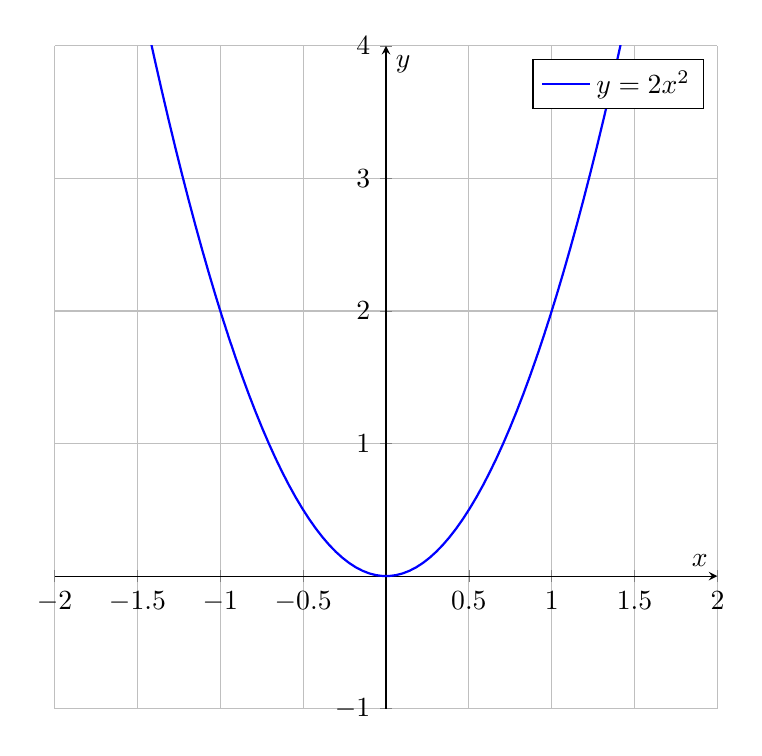
\begin{tikzpicture}
        \begin{axis}[
            axis lines = middle,
            xlabel = $x$,
            ylabel = $y$,
            xmin = -2, xmax = 2,
            ymin = -1, ymax = 4,
            samples = 100,
            width = 10cm,
            height = 10cm,
            grid = both
        ]
        \addplot [
            domain=-2:2,
            color=blue,
            thick
        ]
        {2*x^2};
        \addlegendentry{$y = 2x^2$}
        \end{axis}
    \end{tikzpicture}
\end{center}

\subsection{Ecuación general de la parábola con eje horizontal o vertical}
La ecuación general de una parábola puede escribirse en la forma:
\begin{itemize}
    \item \textbf{Eje vertical}: \((y - k)^2 = 4p(x - h)\)
    \item \textbf{Eje horizontal}: \((x - h)^2 = 4p(y - k)\)
\end{itemize}
Donde \((h, k)\) es el vértice de la parábola, y \( p \) es la distancia desde el vértice al foco.

\subsection{Ecuación de la parábola determinada a partir de condiciones dadas}
Para encontrar la ecuación de una parábola, se pueden utilizar diferentes conjuntos de datos:
\begin{itemize}
    \item \textbf{Conociendo el foco y la directriz}: Si el foco es \((h, k + p)\) y la directriz es \(y = k - p\), la ecuación de la parábola es \((x - h)^2 = 4p(y - k)\).
    \item \textbf{Conociendo tres puntos por los cuales pasa la parábola}: Se pueden utilizar los puntos dados para resolver un sistema de ecuaciones que determine los coeficientes de la ecuación general.
\end{itemize}

\begin{center}
    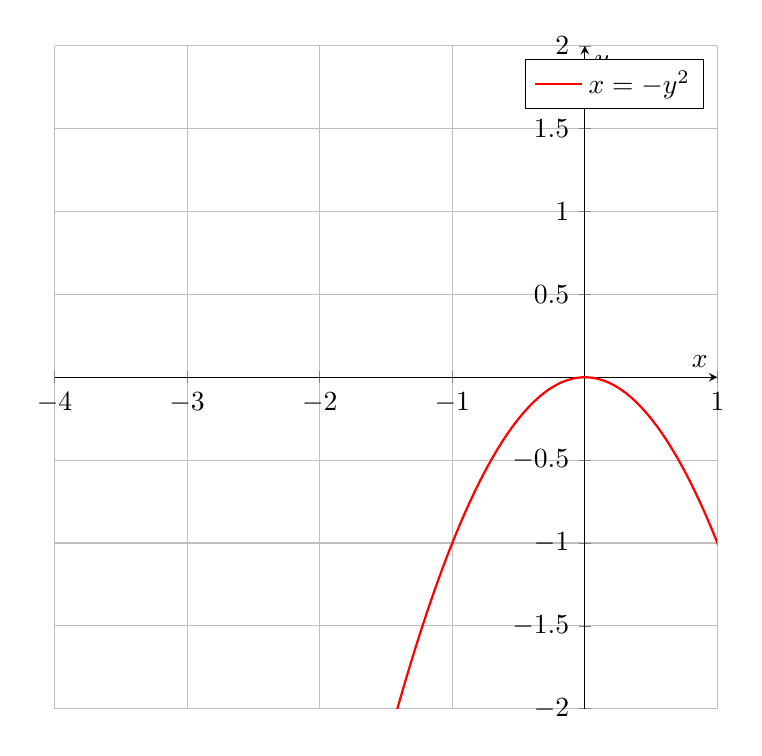
\begin{tikzpicture}
        \begin{axis}[
            axis lines = middle,
            xlabel = $x$,
            ylabel = $y$,
            xmin = -4, xmax = 1,
            ymin = -2, ymax = 2,
            samples = 100,
            width = 10cm,
            height = 10cm,
            grid = both
        ]
        \addplot [
            domain=-2:2,
            color=red,
            thick
        ]
        {-x^2};
        \addlegendentry{$x = -y^2$}
        \end{axis}
    \end{tikzpicture}
\end{center}
\section{Elipse} %(9 horas)

\subsection{Definición de la elipse como lugar geométrico}
Una elipse es el lugar geométrico de los puntos en un plano tal que la suma de las distancias de cada punto a dos puntos fijos, llamados focos, es constante. Es una curva cerrada y simétrica respecto a sus ejes mayor y menor.

\subsection{Ecuación ordinaria de la elipse con ejes paralelos a los ejes de coordenadas y su gráfica respectiva.}
La ecuación ordinaria de una elipse con centro en el origen y ejes mayor y menor paralelos a los ejes de coordenadas es:
\[
\frac{x^2}{a^2} + \frac{y^2}{b^2} = 1
\]
donde \(a\) es el semieje mayor y \(b\) el semieje menor. Si \(a > b\), el eje mayor es horizontal; si \(b > a\), el eje mayor es vertical.

\begin{center}
    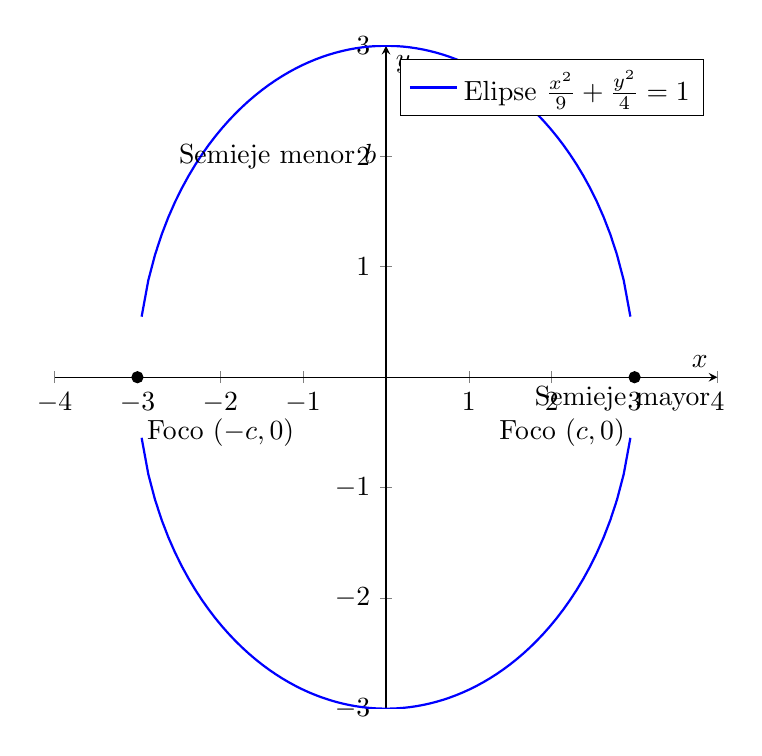
\begin{tikzpicture}
        \begin{axis}[
            axis lines = middle,
            xlabel = $x$,
            ylabel = $y$,
            xmin = -4, xmax = 4,
            ymin = -3, ymax = 3,
            width = 10cm,
            height = 10cm
        ]
        \addplot [
            domain=-4:4,
            samples=100,
            color=blue,
            thick
        ] {sqrt(1 - (x^2/9)) * 3};
        \addplot [
            domain=-4:4,
            samples=100,
            color=blue,
            thick
        ] {-sqrt(1 - (x^2/9)) * 3};
        \addlegendentry{Elipse $\frac{x^2}{9} + \frac{y^2}{4} = 1$}
        \draw [fill] (axis cs:3,0) circle [radius=2pt];
        \node at (axis cs:3,-0.5) [anchor=east] {Foco $(c, 0)$};
        \draw [fill] (axis cs:-3,0) circle [radius=2pt];
        \node at (axis cs:-3,-0.5) [anchor=west] {Foco $(-c, 0)$};
        \node at (axis cs:0,2) [anchor=east] {Semieje menor $b$};
        \node at (axis cs:3,0) [anchor=north] {Semieje mayor $a$};
    \end{axis}
    \end{tikzpicture}
\end{center}

\subsection{Ecuación general de la elipse con eje mayor horizontal o vertical}
La ecuación general de la elipse puede escribirse como:
\[
Ax^2 + By^2 + Cx + Dy + E = 0
\]
donde los coeficientes \(A\) y \(B\) determinan la orientación del eje mayor (horizontal si \(A > B\) y vertical si \(B > A\)).

\subsection{Ecuación de la elipse determinada a partir de condiciones dadas}
Para determinar la ecuación de una elipse a partir de condiciones específicas, se pueden seguir los siguientes pasos:
\begin{enumerate}
    \item Identificar la longitud del semieje mayor \(a\) y del semieje menor \(b\).
    \item Determinar la ubicación del centro de la elipse \((h, k)\).
    \item Utilizar la fórmula \(\frac{(x-h)^2}{a^2} + \frac{(y-k)^2}{b^2} = 1\) para obtener la ecuación.
\end{enumerate}


\section{Hipérbola} %(4.5 horas)

\subsection{Definición de la hipérbola como lugar geométrico}
Una hipérbola es el lugar geométrico de los puntos en un plano tal que el valor absoluto de la diferencia de sus distancias a dos puntos fijos, llamados focos, es constante. Esta constante es igual a la distancia entre los vértices de la hipérbola.

\subsection{Ecuación ordinaria de la hipérbola con centro en el origen de coordenadas}
La ecuación ordinaria de una hipérbola con centro en el origen y ejes asintóticos paralelos a los ejes de coordenadas puede ser de dos tipos:
\begin{itemize}
    \item Con eje transversal horizontal: 
    \[
    \frac{x^2}{a^2} - \frac{y^2}{b^2} = 1
    \]
    \item Con eje transversal vertical:
    \[
    \frac{y^2}{a^2} - \frac{x^2}{b^2} = 1
    \]
\end{itemize}
Donde \(a\) y \(b\) son las longitudes de los semiejes, con \(2a\) siendo la distancia entre los vértices y \(2b\) la distancia entre los focos.

\subsection{Gráfica de la hipérbola}
\begin{center}
    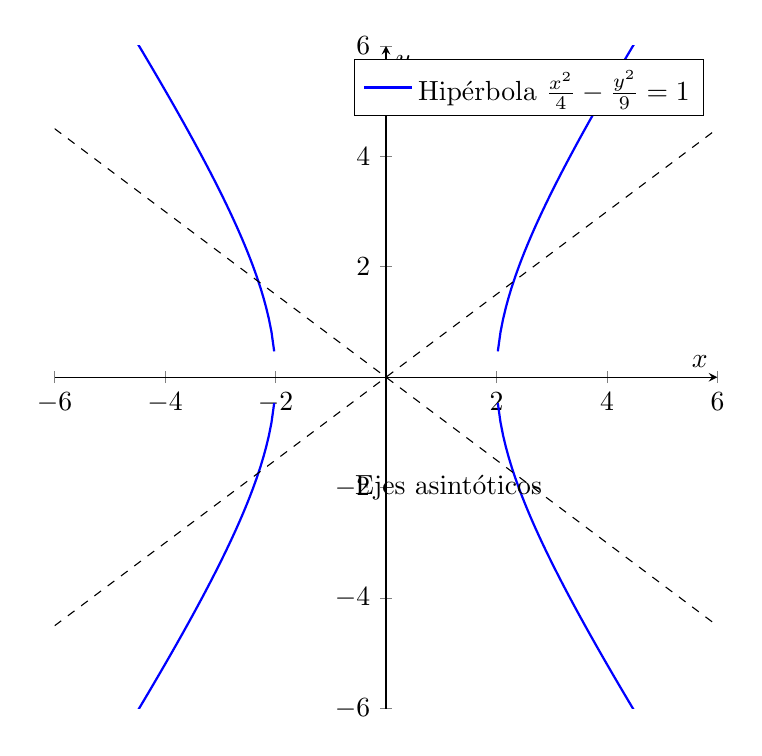
\begin{tikzpicture}
        \begin{axis}[
            axis lines = middle,
            xlabel = $x$,
            ylabel = $y$,
            xmin = -6, xmax = 6,
            ymin = -6, ymax = 6,
            width = 10cm,
            height = 10cm
        ]
        \addplot [
            domain=-6:-1.2,
            samples=100,
            color=blue,
            thick
        ] {sqrt(x^2 / 4 - 1) * 3};
        \addplot [
            domain=1.2:6,
            samples=100,
            color=blue,
            thick
        ] {sqrt(x^2 / 4 - 1) * 3};
        \addplot [
            domain=-6:-1.2,
            samples=100,
            color=blue,
            thick
        ] {-sqrt(x^2 / 4 - 1) * 3};
        \addplot [
            domain=1.2:6,
            samples=100,
            color=blue,
            thick
        ] {-sqrt(x^2 / 4 - 1) * 3};
        \addlegendentry{Hipérbola $\frac{x^2}{4} - \frac{y^2}{9} = 1$}
        
        \draw [dashed] (axis cs:-6,4.5) -- (axis cs:6,-4.5);
        \draw [dashed] (axis cs:-6,-4.5) -- (axis cs:6,4.5);
        \node at (axis cs:3,-2) [anchor=east] {Ejes asintóticos};
    \end{axis}
    \end{tikzpicture}
\end{center}


\section{Lugares geométricos} %(9 horas)

\subsection{Definición}
Un lugar geométrico es un conjunto de puntos que satisfacen una condición geométrica determinada. En geometría analítica, estas condiciones se expresan mediante ecuaciones matemáticas que describen curvas, como líneas rectas, círculos, elipses, parábolas e hipérbolas.

\subsection{Dada una ecuación obtener el lugar geométrico}
Para encontrar el lugar geométrico correspondiente a una ecuación dada, se identifican las características y restricciones que esta ecuación impone sobre los puntos en el plano cartesiano. Por ejemplo, la ecuación de una circunferencia $(x - h)^2 + (y - k)^2 = r^2$ describe un lugar geométrico en el que todos los puntos están a una distancia constante $r$ del centro $(h, k)$.

Ejemplo: Encontrar el lugar geométrico de la ecuación $x^2 + y^2 = 25$.
\begin{itemize}
    \item La ecuación $x^2 + y^2 = 25$ describe una circunferencia con centro en el origen $(0, 0)$ y radio 5.
\end{itemize}

\begin{center}
    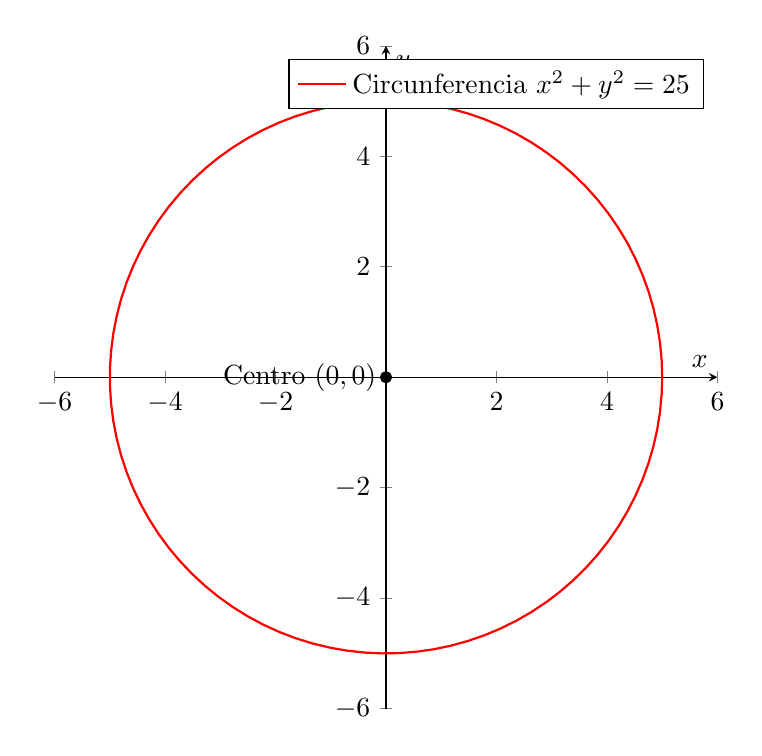
\begin{tikzpicture}
        \begin{axis}[
            axis lines = middle,
            xlabel = $x$,
            ylabel = $y$,
            xmin = -6, xmax = 6,
            ymin = -6, ymax = 6,
            width = 10cm,
            height = 10cm
        ]
        \addplot [
            domain=0:2*pi,
            samples=100,
            color=red,
            thick
        ]
        ({5*cos(deg(x))}, {5*sin(deg(x))});
        \addlegendentry{Circunferencia $x^2 + y^2 = 25$}
        
        \draw [fill] (axis cs:0,0) circle [radius=2pt];
        \node at (axis cs:0,0) [anchor=east] {Centro $(0, 0)$};
    \end{axis}
    \end{tikzpicture}
\end{center}

\subsection{Dado el lugar geométrico obtener la ecuación}
Para determinar la ecuación que corresponde a un lugar geométrico dado, se utilizan las propiedades geométricas del lugar. Esto implica formular una expresión matemática que capture las relaciones geométricas descritas.

Ejemplo: Encuentra la ecuación de una parábola cuyo vértice está en el origen y cuya directriz es la línea $y = -2$.
\begin{itemize}
    \item La ecuación de una parábola con vértice en el origen y directriz $y = -2$ se puede encontrar utilizando la definición de parábola. La distancia de cualquier punto $(x, y)$ en la parábola al foco $(0, 1)$ debe ser igual a su distancia a la directriz $y = -2$. Esto nos lleva a la ecuación:
    \[
    y^2 = 4(x - (-2))
    \]
    o simplificada,
    \[
    y^2 = 4x
    \]
\end{itemize}

\begin{center}
    \begin{tikzpicture}
        \begin{axis}[
            axis lines = middle,
            xlabel = $x$,
            ylabel = $y$,
            xmin = -5, xmax = 5,
            ymin = -5, ymax = 5,
            width = 10cm,
            height = 10cm
        ]
        \addplot [
            domain=-5:5,
            samples=100,
            color=blue,
            thick
        ] {sqrt(4*x)};
        \addplot [
            domain=-5:5,
            samples=100,
            color=blue,
            thick
        ] {-sqrt(4*x)};
        \addlegendentry{Parábola $y^2 = 4x$}
        
        \draw [dashed] (axis cs:-5,-2) -- (axis cs:5,-2);
        \node at (axis cs:3,-2.5) [anchor=north] {Directriz $y = -2$};
    \end{axis}
    \end{tikzpicture}
\end{center}